\section{РУКОВОДСТВО ПОЛЬЗОВАТЕЛЯ}
\label{sec:manual}

%В руководстве пользователя дается описание работы с программой.
%Указываются требования к аппаратному и программному обеспечению.
%Описывается процесс инсталляции с указанием каталогов, ключей реестра, конфигурационных файлов и так далее.
%Также описывается пользовательский интерфейс с указанием элементов управления (пунктов меню, кнопок, закладок и т. д.),
%режимов  работы  и  последовательности  действий.
%Здесь  могут  приводиться скриншоты работы программы.

В данном разделе описана информация, которая необходима пользователям разрабатываемой системы для ее корректного использования.

%Данный дипломный проект будет иметь несколько групп пользователей с разными правами доступа:
%\begin{itemize}
%    \item администратор;
%    \item аналитик;
%    \item трейдер.
%\end{itemize}

Поскольку у продукта отсутствует визуальный интерфейс и другие способы
взаимодействия с системой, дальнейшее описание касается в первую очередь тех людей, кто будет
производить разработку визуальной части веб-приложения, составной частью которого является текущая разработка.

\subsection{Общее описание особенностей}

Разрабатываемая в контексте данного дипломного проекта часть системы поставляется в виде исходных кодов программы.
Так же она может быть передана при помощи контейнеров Docker и способна работать на настольных и серверных операционных системах.
Для возможности запуска контейнеров в системе должен быть установлен Docker.

Так как сборка и запуск происходит посредством платформы Docker то они не зависят от используемых компиляторов и целевых архитектур.

\subsection{Требования к аппаратному и программному обеспечению}

Так как сборка и запуск происходит посредством платформы Docker, то аппаратные требования в первую очередь ограничиваются самой платформой.
На официальном сайте
Для сборки и дальнейшего использования данного дипломного проекта необходимо следующее программное обеспечение:
\begin{itemize}
    \item операционная система, на которой будет производится запуск контейнеров;
    \item установленная платформа Docker для сборки, запуска и перемещения контейнеров;
    \item установленная платформа Docker Compose для инициализации и запуска приложений на основе контейнеров.
\end{itemize}

Основной платформой, которая заявлена в требованиях, является операционная система семейства Linux.
В качестве примера, на котором будет показана установка всех необходимых
зависимостей, была взята Ubuntu 22.04 LTS amd64 как версия одного из самых популярных дистрибутивов на момент написания текущего руководства.

\nomenclaturex{LTS}{Long-Term Support}{увеличенный срок поддержки}

Порядок установки выбранной операционной системы описан в источнике~\cite{ubuntu_how_to_install}.
Несмотря на то, что там расписан порядок установки для более старой версии данного дистрибутива, выбранный вариант полностью соответствует новой версии.
Скачать необходимую версию дистрибутива можно с официального сайта~\cite{ubuntu_download_site}.

\subsubsection{Установка Docker на операционную систему Linux}

После установки операционной системы необходимо установить платформу Docker.
Сделать это можно из терминала с помощью следующих команд:

\begin{lstlisting}[basicstyle=\ttfamily\small]
$ sudo apt update
$ sudo apt install curl software-properties-common ca-certificates apt-transport-https -y
$ wget -O- https://download.docker.com/linux/ubuntu/gpg | gpg --dearmor | sudo tee /etc/apt/keyrings/docker.gpg > /dev/null
$ echo "deb [arch=amd64 signed-by=/etc/apt/keyrings/docker.gpg] https://download.docker.com/linux/ubuntu jammy stable"| sudo tee /etc/apt/sources.list.d/docker.list > /dev/null
$ sudo apt update
$ apt-cache policy docker-ce
$ sudo apt install docker-ce -y
\end{lstlisting}

Проверить установку платформы Docker можно при помощи следующей команды:

\begin{lstlisting}[basicstyle=\ttfamily\small]
$ sudo systemctl status docker
\end{lstlisting}

Указанные команды установят все необходимые для запуска сборки зависимости.
Для корректной работы рекомендуется перезапустить терминал или весь персональный компьютер.

\subsubsection{Установка Docker на операционную систему Windows}

Для начала требуется скачать установщик, который можно найти на странице официального сайта~\cite{docker_download}.
\\
После окончания загрузки установщика требуется его запустить, дважды кликнув по Docker Desktop Installer.exe.
\\
Убедитесь, что в конфигурации выбран параметр «Использовать WSL 2 вместо Hyper-V» или нет, в зависимости от выбора серверной части.
Если опереационная система, на которую устанавливается платформа Docker, поддерживает только один из двух вариантов,
выбрать, какой сервер использовать, не будет возможным.

Далее требуется следовать инструкциям мастера установки, разрешив установщику вносить изменения, и продолжить установку.

После успешной установки выберите «Закрыть», чтобы завершить процесс установки.

Если учетная запись администратора отличается от учетной записи пользователя, требуется добавить пользователя в группу docker-users:
\begin{enumerate_num}
    \item Запустите «Управление компьютером от имени администратора».
    \item Перейдите в раздел «Локальные пользователи и группы» > «Группы» > «docker-users».
    \item Щелкните правой кнопкой мыши, чтобы добавить пользователя в группу.
    \item Выйдите из системы и войдите снова, чтобы изменения вступили в силу.
\end{enumerate_num}

\subsection{Запуск прилложения}

Как было сказано выше, разработанное приложение работает внутри системы Docker.
Система разделена на два микросервиса, каждый из которых содержит файл Dockerfile, поэтому запуск происходит для каждого микросервиса отдельно.

\subsubsection{Создание сети Docker}

Для того чтобы микросервисы смогли взаимодействовать, их требуется запускать в одной сети Docker.
Данная сеть указана в файле docker-compose.yml для каждого микросервиса, однако её требуется создать средствами Docker.
Для того чтобы создать сеть Docker можно воспользоваться следующей командой в терминале:

\begin{lstlisting}[basicstyle=\ttfamily\small]
$ docker network create -d bridge fastapi_kafka
\end{lstlisting}
В данной коменде указано название сети, соответствующее названию из файлов docker-compose.yml.
Для того чтобы связать виртуальные порты внутри сети Docker с реальными портами компьютера требуется изменить тип сети с bridge на host,
однако это может подвергнуть безопасность системы, поэтому при развертывании приложения в глобальной сети рекомендуется воспользоваться средствами Kubernetes.

\subsubsection{Сборка контейнеров Docker}

Для сборки контейнеров требуется перейти в терминале в корневой каталог проекта, в котором находится файл docker-compose.yml.

Для сборки можно воспользоваться следующей командой:
\begin{lstlisting}[basicstyle=\ttfamily\small]
$ docker-compose build
\end{lstlisting}

\subsubsection{Запуск контейнеров Docker}

Для запуска приложения требуется воспользоваться следующей командой:
\begin{lstlisting}[basicstyle=\ttfamily\small]
$ docker-compose up
\end{lstlisting}
Для того чтобы запустить приложение в фоновом режиме без вывода логов можно добавить флаг -d.

Для просмотра запущенных контейнеров требуется воспользоваться следующей командой:
\begin{lstlisting}[basicstyle=\ttfamily\small]
$ docker-compose ps
\end{lstlisting}

Для приостановки приложения требуется воспользоваться следующей командой:
\begin{lstlisting}[basicstyle=\ttfamily\small]
$ docker-compose stop
\end{lstlisting}

Для полной остановки требуется воспользоваться следующей командой:
\begin{lstlisting}[basicstyle=\ttfamily\small]
$ docker-compose down
\end{lstlisting}
Однако следует быть осторожным в применении данной команды, так как она очищает все данные, связанные с контейнерами.

\subsection{Документация}\label{subsec:manual:docs}

Документация для разработчиков доступна в виде аннотаций типов и строк документации прямо в исходном коде.

Для визуализации доступного функционала приложения предлагается воспользоваться средствами Swagger,
реализованного в данном проекте при помощи интеграции библиотеки drf-spectacular.

Swagger -- это фреймворк для спецификации REST API.
Главным плюсом является то, что он дает возможность не только интерактивно просматривать спецификацию, но и отправлять запросы.
Данная технология именуется как Swagger UI и формирует представления на основании исходного кода приложения.
Отображение документации доступного функционала при помощи Swagger UI показано на рисунке~\ref{fig:manual:swagger1}.

\begin{figure}[ht]
    \centering
    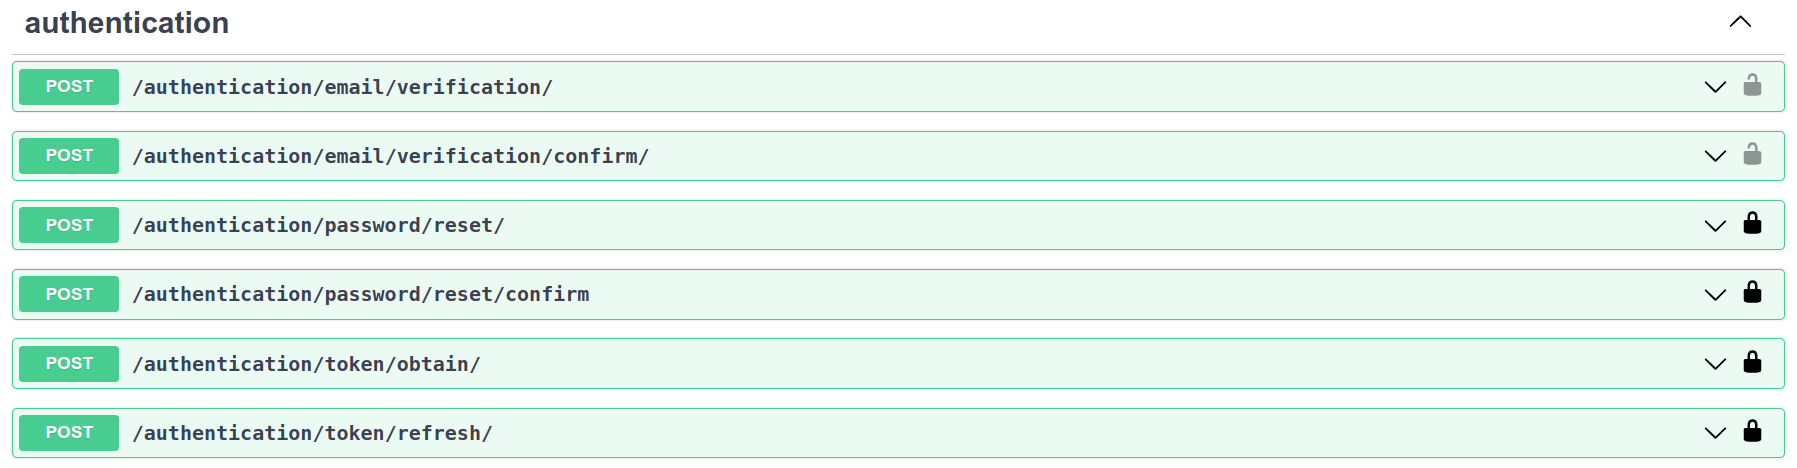
\includegraphics[width=.9\linewidth]{images/swagger1}
    \caption{Отображение эндпоинтов в Swagger UI}
    \label{fig:manual:swagger1}
\end{figure}


\nomenclaturex{UI}{User Interface}{пользовательский интерфейс}





%
%Установка сред разработки для целевых платформ FreeRTOS и TI-RTOS описана в официальной документации~\cite{st_cubeide_install} и~\cite{ti_ccs_install} соответственно.
%Порядок установки TI-RTOS SDK для семейства AM57xx также предоставлен его разработчиками~\cite{ti_sdk_install}.
%
%\subsection{Сборка исходных кодов}
%
%Для сборки разработанной библиотеки необходимо скопировать ее с диска, поставляемого
%с дипломным проектом, на компьютер. Сделать это можно как средствами
%графического интерфейса, так и с помощью утилит командной строки.
%
%Поставляемые пакеты необходимо собирать в следующем порядке для корректного
%разрешения зависимостей:
%\begin{enumerate_num}
%    \item OsalApi.
%    \item Shared.
%    \item OSAL для операционной системы Linux.
%    \item libiec61850.
%    \item libxml2.
%    \item GooseReceiver.
%\end{enumerate_num}
%
%Сборка пакетов в ином порядке может привести к получению ошибок
%отсутствия зависимостей или использованию их старых версий.
%Поскольку сборка каждого компонента выполняется идентично, она будет
%продемонстрирована на примере одного из них.
%
%Предположим, что пользователь поместил скопированные файлы в директорию
%\lstinline{$HOME/dvd}. Для выполнения сборки пакета Shared
%под Linux необходимо выполнить следующие действия в терминале:
%
%\begin{lstlisting}
%$ cd "$HOME/dvd"
%$ export CI_COMMIT_TAG="1.0.0"
%$ export CONAN_REMOTE_USER_OR_URL_SUFFIX="goose-receiver-prj"
%$ cd Shared
%$ CUSTOM_CONAN_PROFILE=x86_64.gcc11.conf CUSTOM_CONAN_BUILD_TYPE=Release ./scripts/conan-run.py
%\end{lstlisting}
%
%Рассмотрим подробнее ключевые моменты, которые были сделаны в процессе сборки.
%Переменная \lstinline{CI_COMMIT_TAG} указывает версию, которая будет присвоена
%пакету. Указанная версия должна быть совместима как со способами нумерации
%пакетов в Conan, так и нумерацией пакетов в CMake, поскольку это значение
%используется обоими инструментами.
%
%Переменная \lstinline{CONAN_REMOTE_USER_OR_URL_SUFFIX} указывает
%Conan название проекта, к которому он будет относить собираемые библиотеки.
%При использовании пакетов локально имя может быть любым, которое будет
%соответствовать требованиям системы сборки. В случае работы с удаленным
%сервером необходимо указывать имя проекта на сервере Conan для
%возможности успешного сохранения скомпилированных библиотек на этот сервер.
%
%Переменная \lstinline{CUSTOM_CONAN_PROFILE} описывает файл, который
%содержит информацию о
%целевой системе, наборе инструментов и окружении для сборки исходных кодов.
%По своей задумке Conan является универсальным пакетным менеджером,
%а на практике поддерживает только самые популярные платформы и архитектуры
%персональных компьютеров и серверов. Поэтому для обхода этого ограничения
%для всех встраиваемых платформ целевой операционной системой является Arduino.
%В некоторых случаях архитектура и компиляторы также указываются некорректно из-за
%отсутствия их поддержки по умолчанию.
%
%\begin{table}[ht]
%    \caption{Возможные типы сборки Conan и CMake}
%    \label{table:manual:buildTypes}
%    \begin{tabular}{| >{\raggedright}m{0.27\textwidth}
%                    | >{\raggedright\arraybackslash}m{0.677\textwidth}|}
%        \hline
%        \centering Название & \centering\arraybackslash Описание \\
%
%        \hline
%        Debug &
%        Отладочная сборка
%        \\
%
%        \hline
%        Release &
%        Сборка для выпуска
%        \\
%
%        \hline
%        RelWithDebInfo &
%        Сборка для выпуска с отладочной информацией
%        \\
%
%        \hline
%        MinSizeRel &
%        Сборка для выпуска с минимизацией размера
%        \\
%
%        \hline
%    \end{tabular}
%\end{table}
%
%\fixTableSectionSpace
%
%\begin{figure}[ht]
%    \centering
%    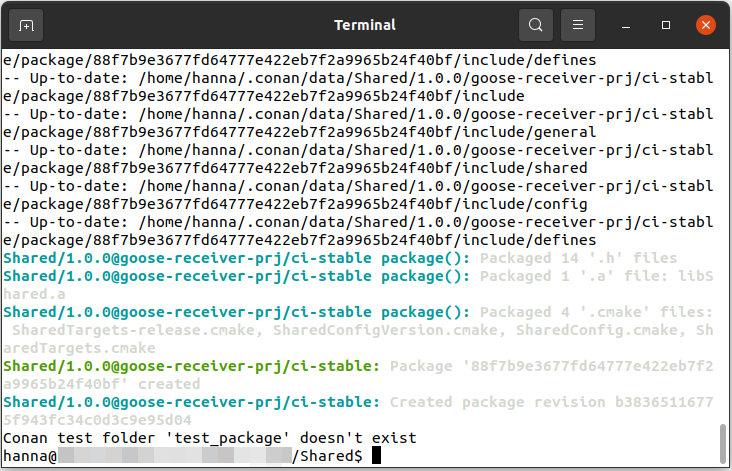
\includegraphics[width=0.8\linewidth]{SharedPackageBuildLog}
%    \caption{Результаты сборки пакета Shared}
%    \label{pic::manual::sharedPkgBuild}
%\end{figure}
%
%Переменная \lstinline{CUSTOM_CONAN_BUILD_TYPE} описывает тип сборки, возможные
%значения и описание которых приведены в таблице~\ref{table:manual:buildTypes}.
%Эти значения совпадают для Conan и CMake, который вызывается
%Conan. Каждый из перечисленных вариантов преследует различные цели.
%Так, например, вариант Release ориентирован на минимизацию времени исполнения кода,
%тогда как MinSizeRel может пожертвовать скоростью работы в пользу меньшего
%размера итогового файла.
%В итоге каждый из приведенных типов сборки соответствует определенным наборам флагов
%компилятора и в некоторых случаях компоновщика для достижения максимальной
%эффективности.
%Переопределить флаги можно в файле опций набора инструментов, который
%используется CMake.
%
%В результате сборки должен появиться вывод, аналогичный
%рисунку~\ref{pic::manual::sharedPkgBuild}.
%
%После успешной сборки вспомогательных пакетов необходимо произвести компиляцию
%платформозависимого кода для операционной системы Linux. Это необходимо
%сделать для проведения тестирования остальных пакетов на текущем компьютере.
%Выполнение описанных ниже команд в терминале произведут необходимую сборку.
%В результате будет получен вывод, аналогичный
%рисунку~\ref{pic::manual::osalPkgBuild}.
%
%\begin{lstlisting}
%$ cd "$HOME/dvd"
%$ export CI_COMMIT_TAG="1.0.0"
%$ export CONAN_REMOTE_USER_OR_URL_SUFFIX="goose-receiver-prj"
%$ cd OSAL
%$ CUSTOM_CONAN_PROFILE=x86_64.gcc11.conf CUSTOM_CONAN_BUILD_TYPE=Release ./scripts/conan-run.py
%\end{lstlisting}
%
%\fixTableSectionSpace
%
%\begin{figure}[ht]
%    \centering
%    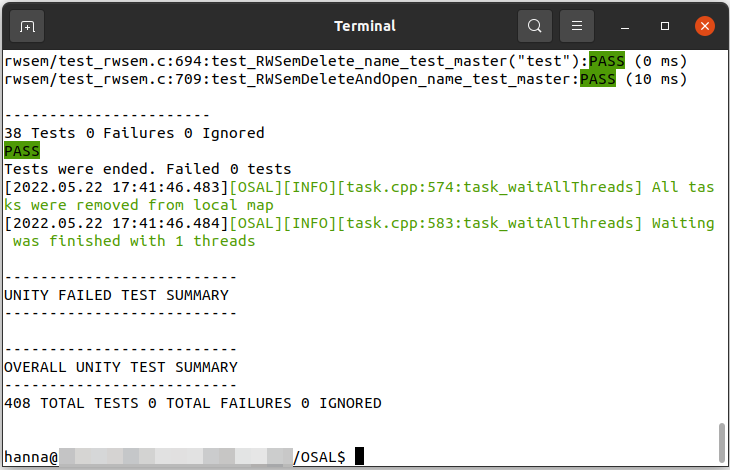
\includegraphics[width=0.8\linewidth]{OsalPackageBuildLog}
%    \caption{Результаты сборки и тестирования пакета OSAL}
%    \label{pic::manual::osalPkgBuild}
%\end{figure}
%
%\fixTableSectionSpace
%
%\subsection{Автоматизированное тестирование}
%
%Если посмотреть вывод скрипта сборки на рисунке~\ref{pic::manual::osalPkgBuild},
%то можно увидеть результаты прохождения
%тестирования под операционную систему Linux.
%Отключение автоматического исполнения тестов можно произвести с помощью приведенной ниже
%команды в терминале, из которого выполняется сборка.
%
%\begin{lstlisting}
%$ export GITLAB_CI=1
%\end{lstlisting}
%
%В результате выполнения этой команды последующие сборки из этого терминала
%будут пропускать этап исполнения тестов.
%
%Если по умолчанию запуск тестов не производится, то существует несколько
%возможных вариантов:
%\begin{itemize}
%    \item происходит кросс-компиляция -- сборка под другую целевую архитектуру или операционную систему;
%    \item отключено исполнение тестов описанным выше способом.
%\end{itemize}
%
%В первом случае ничего изменить не получится, поскольку запустить
%тесты другой аппаратной или программной платформы без эмуляции не представляется
%возможным.
%Во втором же случае поведение можно вернуть на ожидаемое выполнением следующей
%команды:
%
%\begin{lstlisting}
%$ export GITLAB_CI=
%\end{lstlisting}
%
%В результате в текущем терминале выполнение тестов после их сборки
%будет возобновлено.
%
%\subsection{Интеграция со средой разработки}
%
%Для того, чтобы иметь возможность собирать проекты с помощью
%интегрированной среды разработки и подтягивать необходимые
%библиотеки из Conan, необходимо в настройки компилятора добавить
%файл с настройками сборки и связывания из Conan и CMake.
%
%Файл с опциями командной строки для компиляции исходных кодов имеет название
%\lstinline!conan.ide.${CMAKE_SYSTEM_PROCESSOR}.include.opt!,
%настройки компоновщика располагаются в
%\lstinline!conan.ide.${CMAKE_SYSTEM_PROCESSOR}.link.opt!.
%Содержимое директории \lstinline!conan.ide.out/ide/! создается путем вызова скрипта
%сборки под необходимый целевой процессор и содержит описанные выше файлы.
%
%Все пути приведены относительно корневой директории конкретного пакета, такой как
%OSAL, Shared или GooseReceiver.
%\lstinline!${CMAKE_SYSTEM_PROCESSOR}! является переменной CMake и
%описывает имя процессора, под который будет производится сборка.
%Обычно ее значение хранится в файле с настройками используемого набора инструментов
%для CMake. Отличие данной переменной от значения, записанного в
%\lstinline!${CMAKE_HOST_SYSTEM_PROCESSOR}!, приведет к выполнению
%кросс-компиляции.
%
%Для набора инструментов GCC добавление нескольких настроек компиляции делается с помощью
%опции командной строки
%\lstinline`@file.opt`, настроек связывания -- \lstinline`-Wl,-Tfile.opt`.
%В обоих случаях приведен пример по добавлению файла \lstinline`file.opt`.
%Вместо этого значения имени файла необходимо использовать тот,
%который содержит настройки текущей целевой архитектуры и операционной
%системы и располагается по указанному ранее пути.
%Принадлежность к ним можно определить с помощью имени файла.
%Расширение \lstinline{.include.opt} соответствует настройкам компиляции,
%\lstinline{.link.opt} -- связывания.
%
%Добавление настроек наборов инструментов конкретной среды разработки
%обычно производится путем взаимодействия с ее графическим интерфейсом.
%Обычно группы настроек компиляции не поддерживаются как отдельная категория и представлена в разделе дополнительных или расширенных
%опций с помощью возможности явного указания флагов, которые будут переданы
%компилятору.
%Набор настроек связывания обычно поддерживается графическими интерфейсами
%в качестве конкретной опции, поскольку для корректной работы встраиваемых систем
%их необходимо связывать с помощью специальных файлов с настройками различных секций
%и доступной памяти.
%
%В случае необходимости получения опций командной строки
%для добавления файлов с настройками сборки и связывания
%других наборов инструментов
%обратитесь к руководству пользователя, которое предоставлено его разработчиками.
